
Grazie alle scelte tecnologiche con cui sono stati implementati i diversi componenti, il prodotto software può essere utilizzato ovunque e sulla maggior parte dei sistemi operativi, sia desktop (Windows, MacOs, Linux), sia mobile (Android o iOs), rispettando il requisito non funzionale della portabilità richiesto dal cliente.\todo{Davide chiede: "Si scrive così iOs?"}
\todo{Davide dice: nella documentazione non mi fa vedere ò sul può ma nel testo c'è... boh non capisco perchè. Lo stesso lo fa con le è accentate che sembrano scomparire. }
L'applicativo si compone di quattro macro componenti:
\begin{itemize}
	\item \textbf{Web Server Spring}: questa componente è in esecuzione su una istanza di Azure Spring Clound e di conseguenza è sempre accessibile dall'applicazione client;
	\item \textbf{Database MySQL}: anch'esso in esecuzione su una istanza di Azure MySQL;
	\item \textbf{Data Collector e Data Analyzer}: queste due applicazioni sono in esecuzione su un Rapsberry Pi 4;
	\item \textbf{Applicazione Client}: grazie al framework Qt, tale applicazione può essere compilata ed eseguita su gran parte dei sistemi operativi. Infatti, l'unica cosa che deve fare l'utente è installare l'APK sul proprio telefono, oppure installare l'applicazione sul proprio computer e lanciarla all'occorrenza. In questo modo, l'utente può accedere ed utilizzate l'applicazione ed i servizi offerti in qualunque momento. 
\end{itemize}

In figura \ref{fig:qtApp}a viene mostrata la schermata di login dell'applicazione. Per accedere alle funzionalità, l'utente deve inserire lo username e la password che gli sono stati fornite dal coordinatore. 
Dopo aver inserito le credenziali, l'utente accede alla dashboard (figura \ref{fig:qtApp}b) in cui è possibile osservare alcune informazioni sul proprio account ed una mappa che mostra la posizione dell'area di appartenenza.
Nel menù laterale è possibile scegliere quali funzionalità utilizzare (figura \ref{fig:qtApp}c): si possono visualizzare informazioni meteorologiche (figura \ref{fig:qtApp}e), allarmi (figura \ref{fig:qtApp}d) o informazioni sul proprio account e sul proprio team, compresi alcuni dati sui membri del team (figura \ref{fig:qtApp}f).

Il coordinatore potrà invece scegliere dei servizi diversi da quelli di un utente normale (figura \ref{fig:qtApp2}a). Infatti, tale figura ha il compito di inserire nuovi volontari inserendone i dati (figura \ref{fig:qtApp2}b), creare nuove squadre e cancellare degli utenti (figura \ref{fig:qtApp2}c).
\todo{Da rileggere}

\begin{figure}[h!]
	\centering
	\subfloat[\centering Schermata di Login.]{{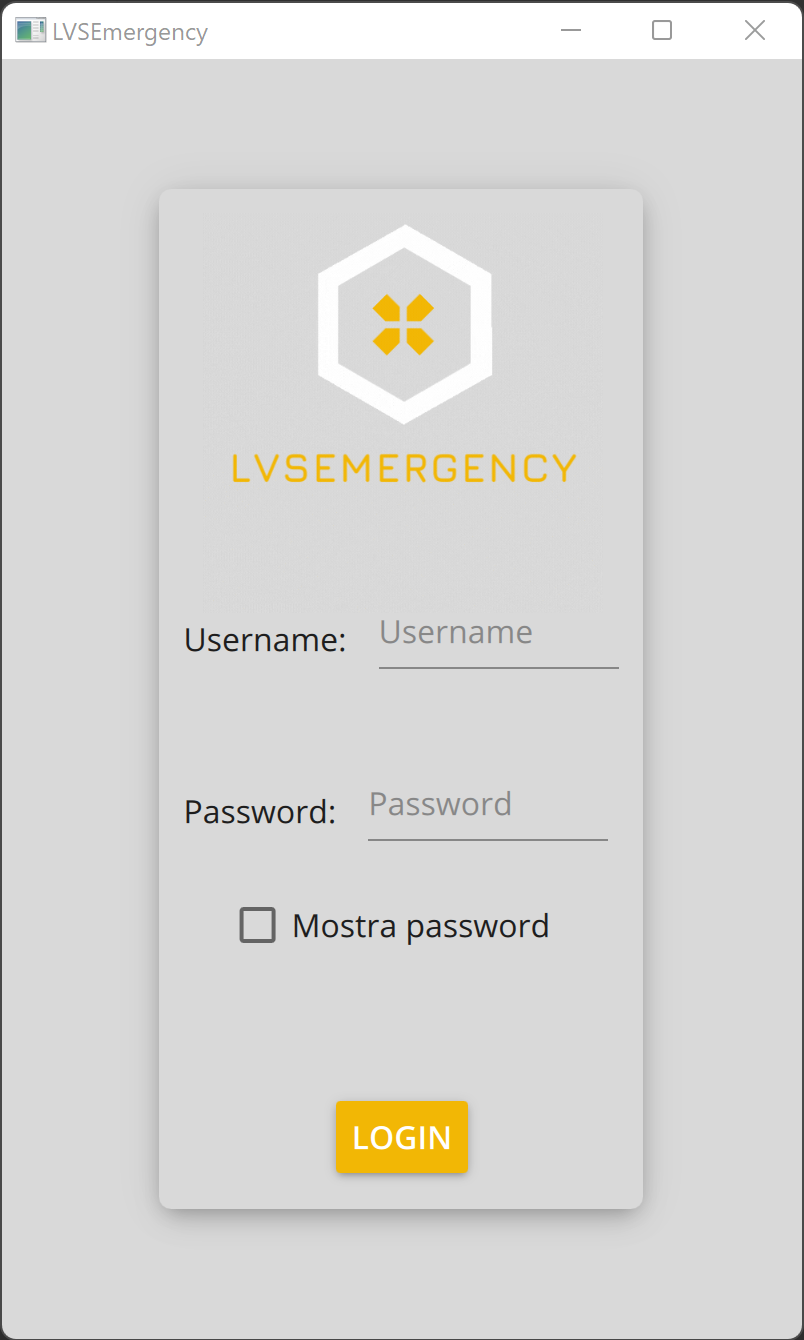
\includegraphics[width=4cm]{./Conclusione/ImageFiles/Login} }}%
	\qquad
	\subfloat[\centering Dashboard.]{{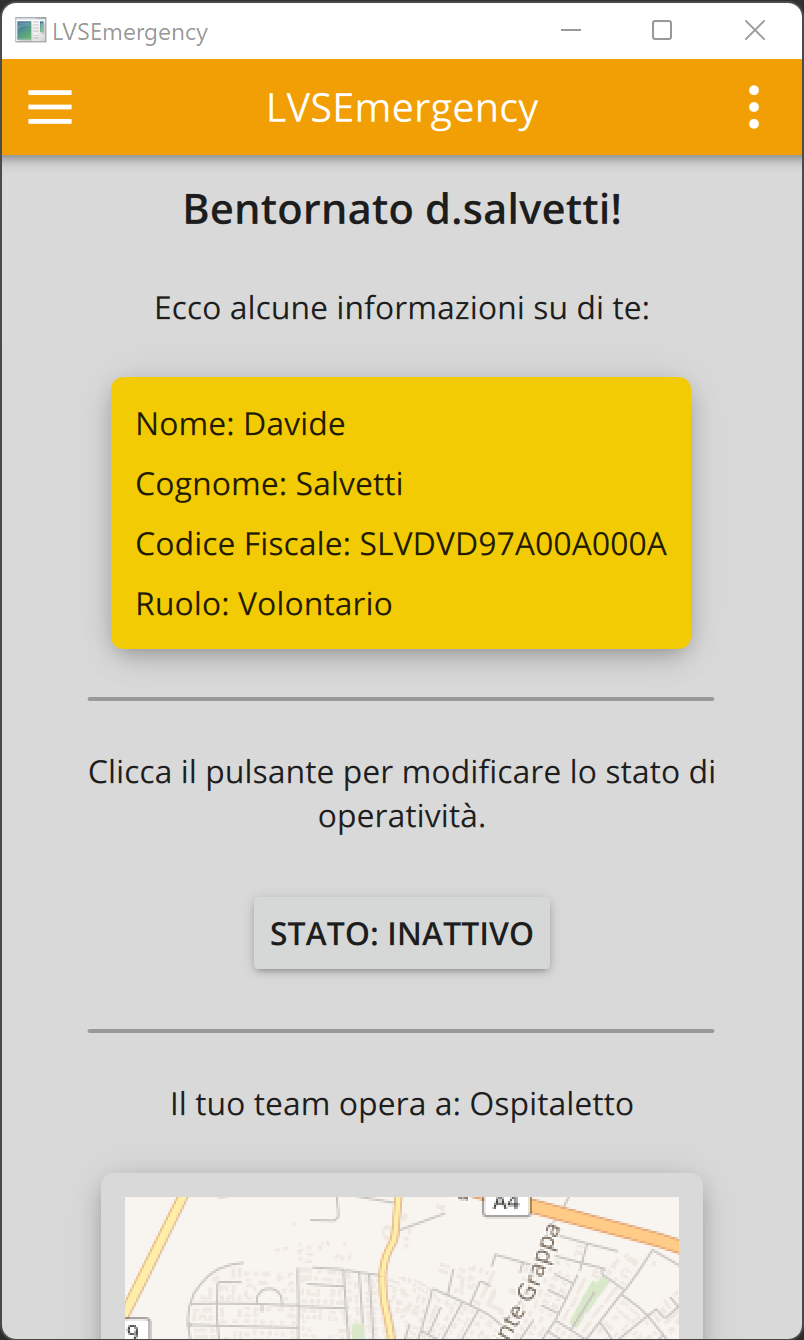
\includegraphics[width=4cm]{./Conclusione/ImageFiles/dashboard} }}%
	\qquad
	\subfloat[\centering Pannello laterale.]{{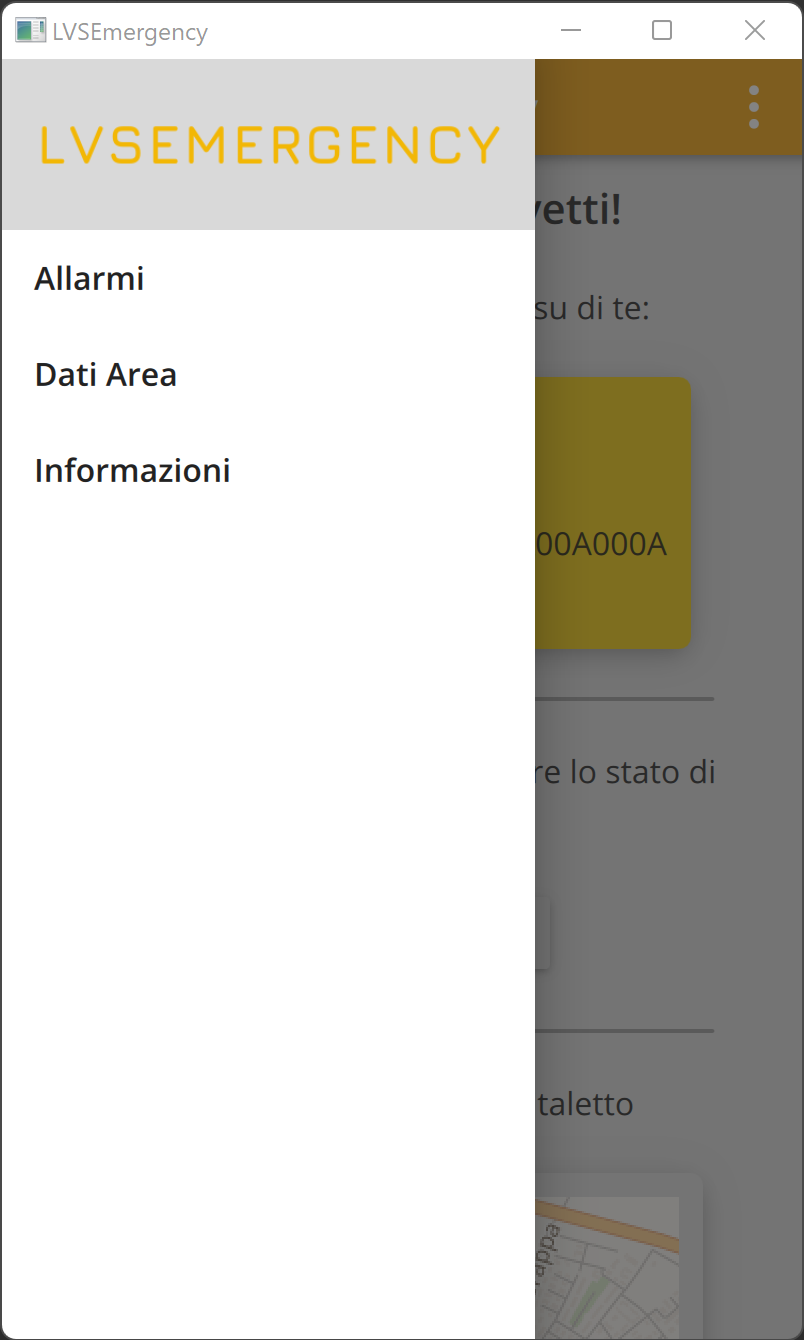
\includegraphics[width=4cm]{./Conclusione/ImageFiles/LateraleUtente} }}%
	\qquad
	\subfloat[\centering Allarmi.]{{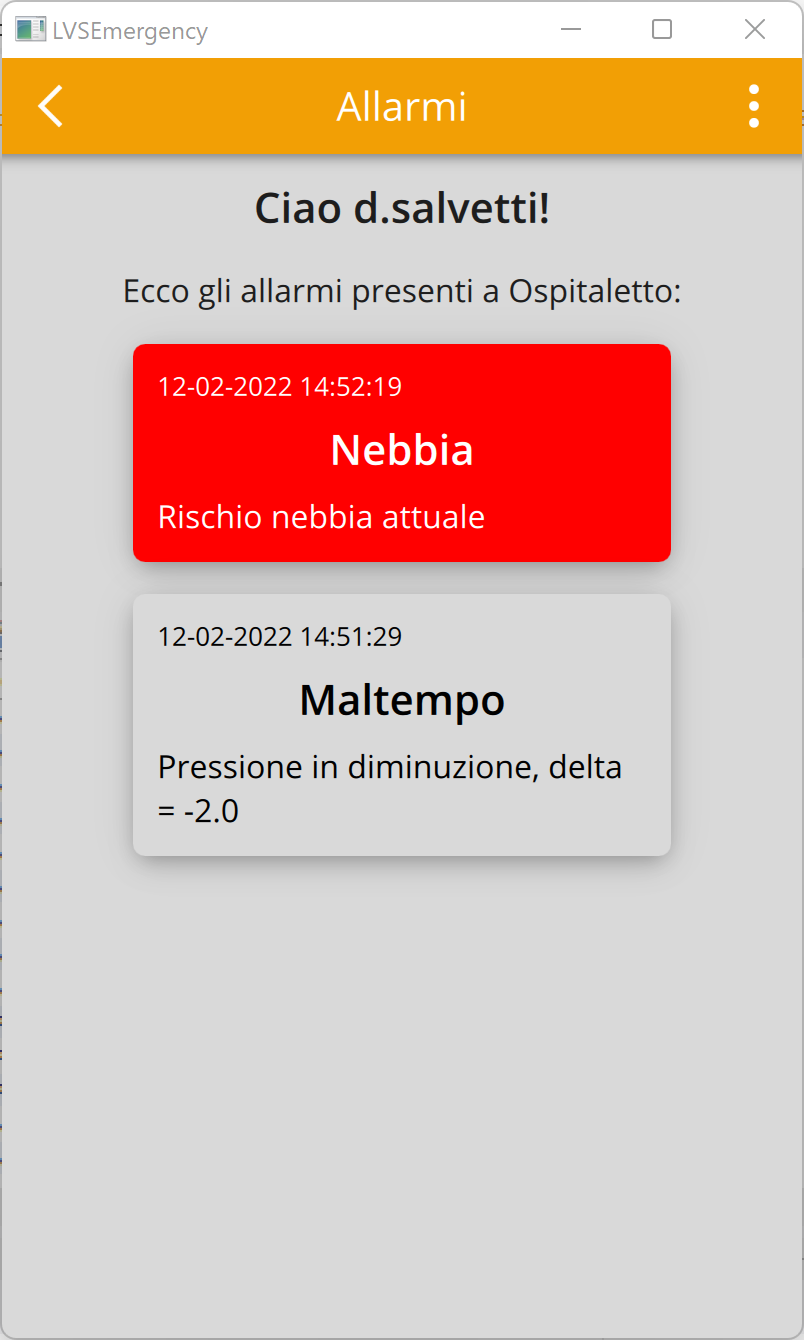
\includegraphics[width=4cm]{./Conclusione/ImageFiles/allarmi} }}%
	\qquad
	\subfloat[\centering Dati meteorologici.]{{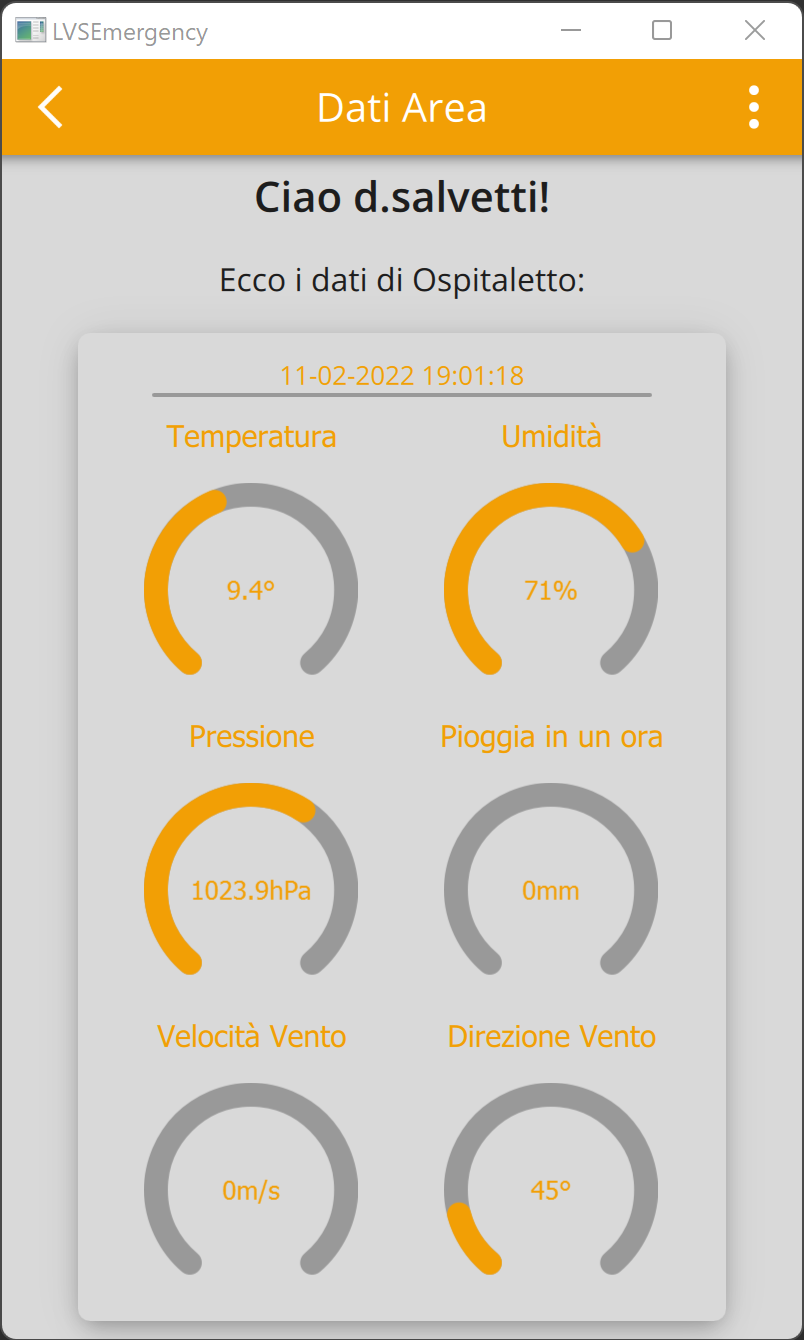
\includegraphics[width=4cm]{./Conclusione/ImageFiles/dati} }}%
	\qquad
	\subfloat[\centering Informazioni utente.]{{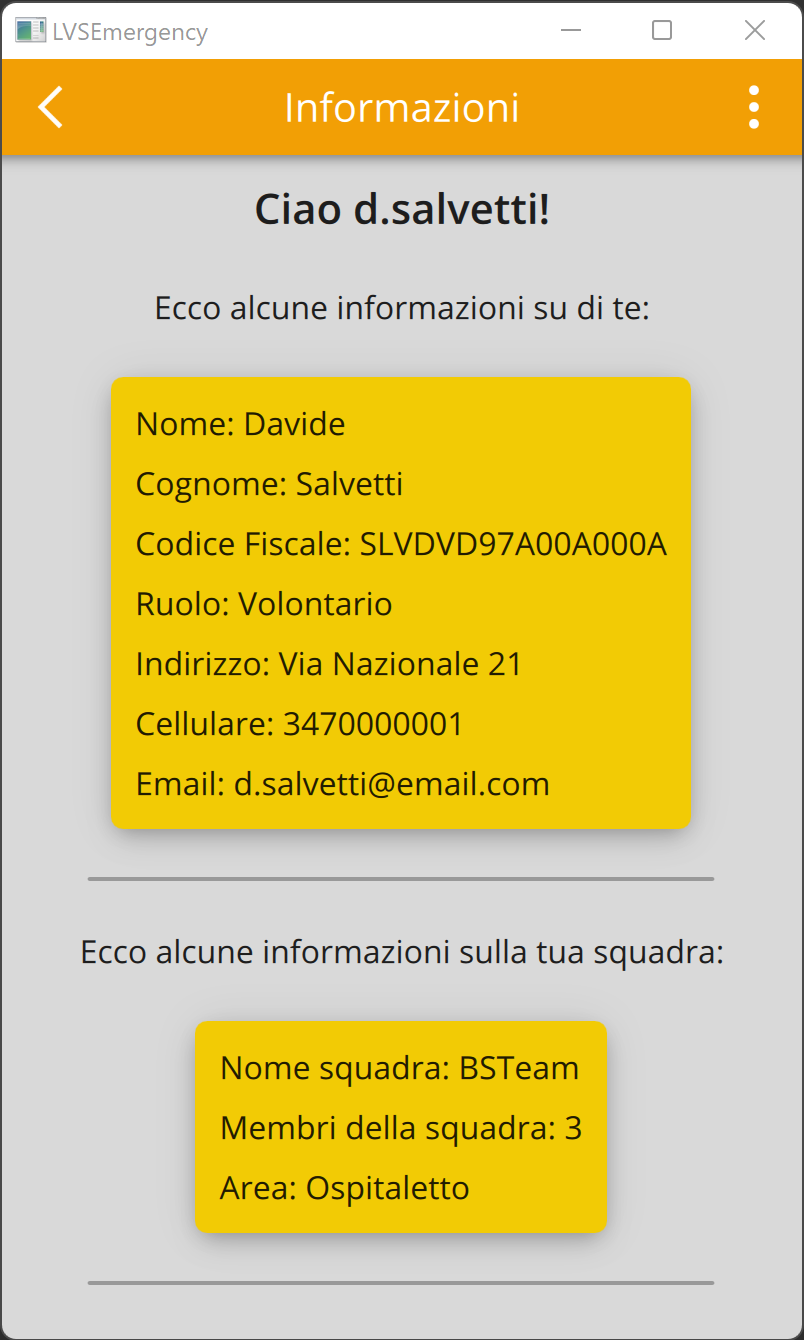
\includegraphics[width=4cm]{./Conclusione/ImageFiles/info1} }}%
	\caption{Funzionalità accessibili da volontari e caposquadra.}%
	\label{fig:qtApp}
\end{figure}


\begin{figure}[h!]
	\centering
	\subfloat[\centering Pannello laterale del coordinatore.]{{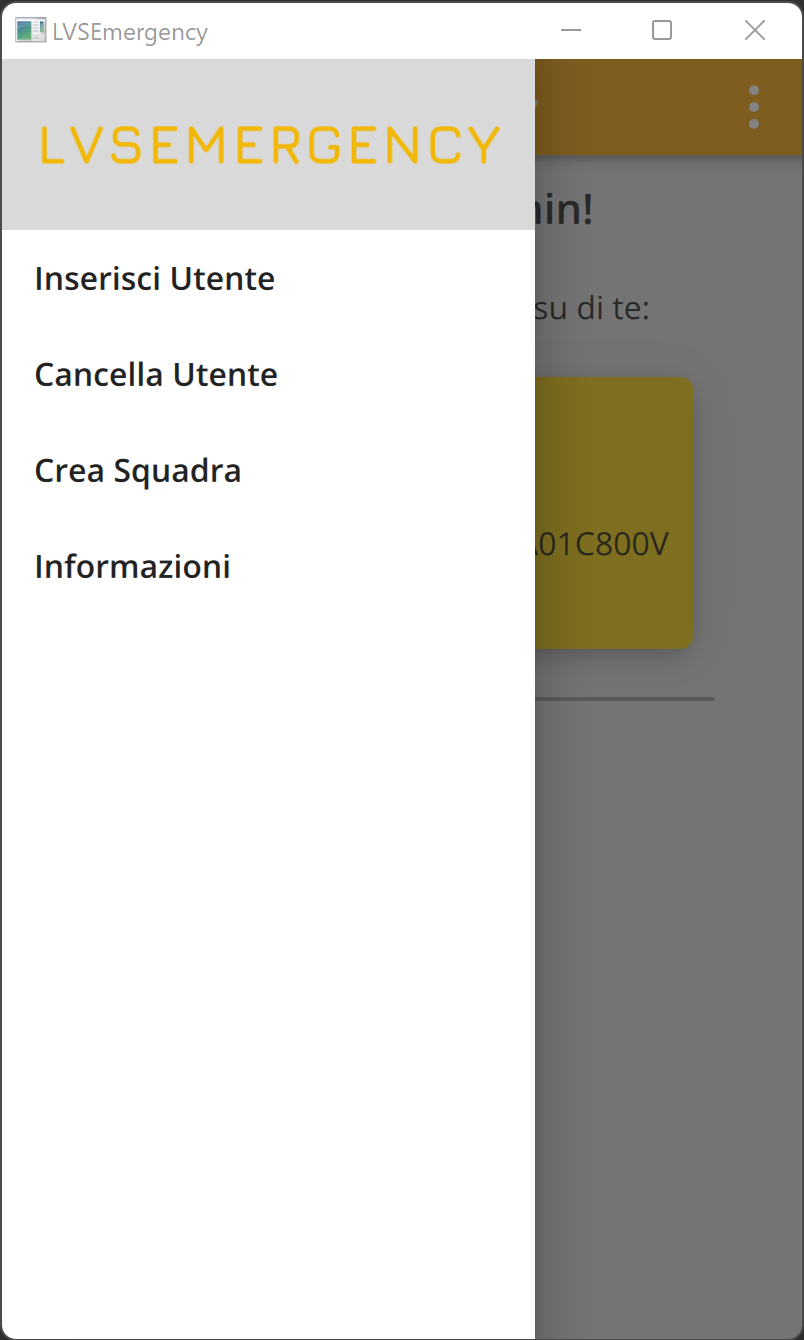
\includegraphics[width=4cm]{./Conclusione/ImageFiles/LateraleAdmin} }}%
	\qquad
	\subfloat[\centering Inserisci utente.]{{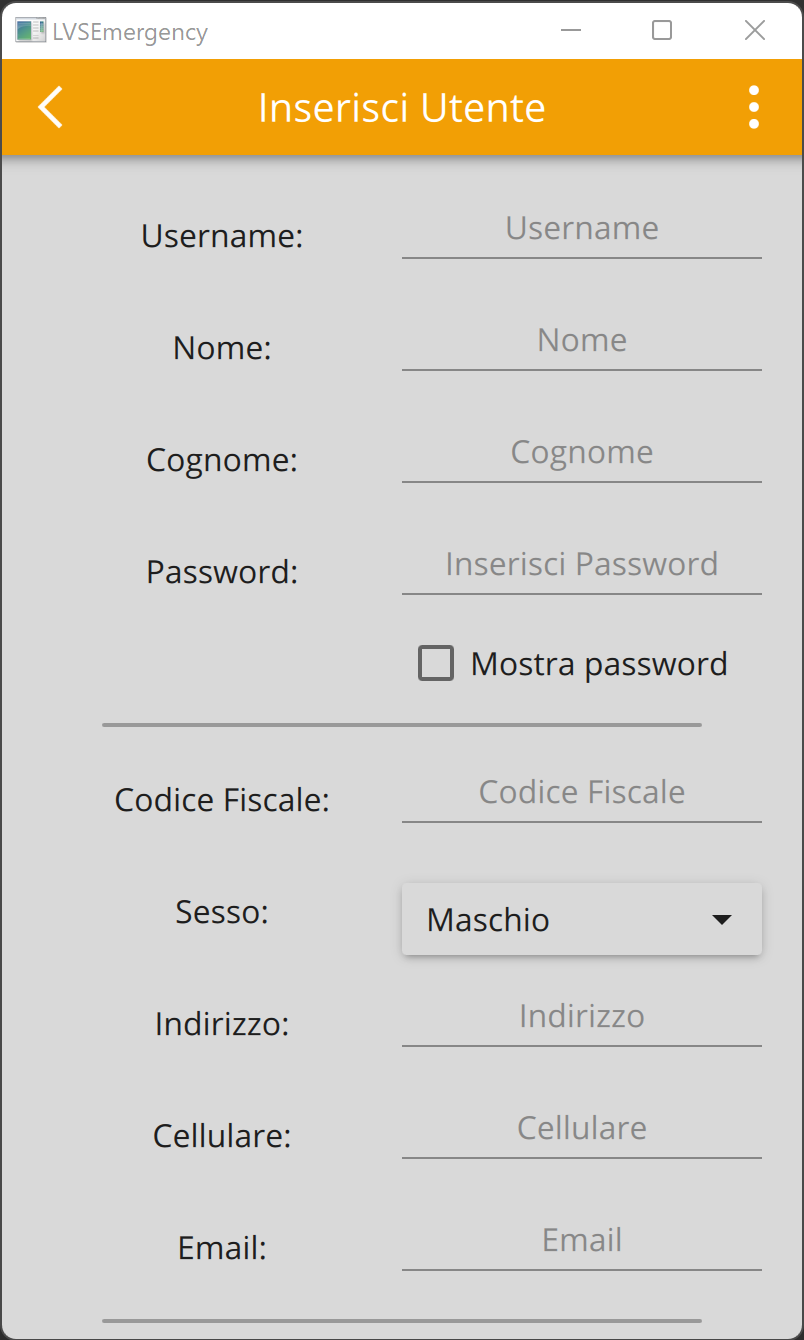
\includegraphics[width=4cm]{./Conclusione/ImageFiles/inserisciUtente} }}%
	\qquad
	\subfloat[\centering Cancella utente.]{{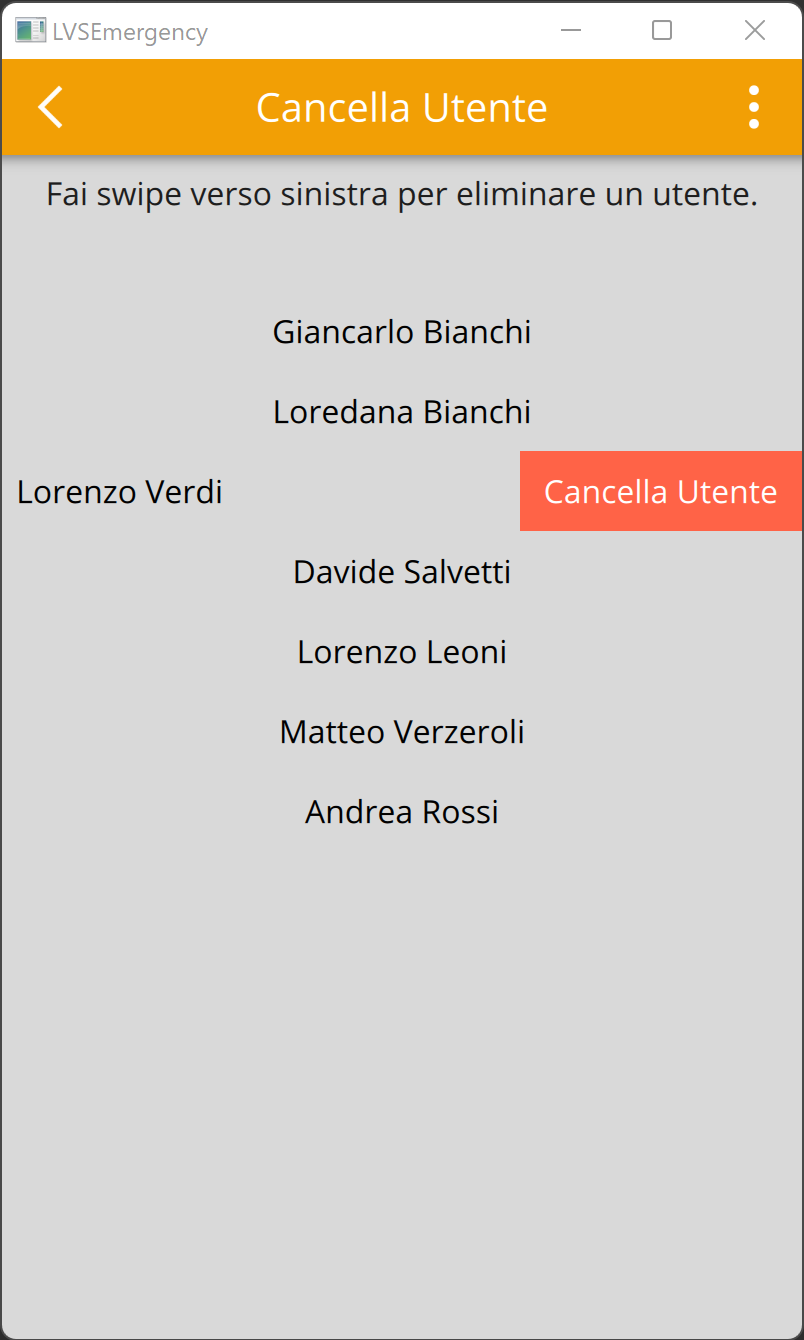
\includegraphics[width=4cm]{./Conclusione/ImageFiles/cancellaUtente} }}%
	\caption{Funzionalità accessibili dai coordinatori.}%
	\label{fig:qtApp2}
\end{figure}


